\chapter{Background}
\label{bgch}

This chapter provides information relevant to the core parts of this research, with 
a particular focus on areas relevant to the novel work presented. We start by 
discussing the two main approaches to solving the NTE, Monte Carlo methods and 
deterministic methods, as the hybrid methods that are described next incorporate both
types of solutions. Then, a discussion of previous work in the field of hybrid methods
is given, with a specific focus on the CADIS method and variants on that method as
well as significant historical work that has incorporated angular information into
hybrid methods. Finally, we present a mathematical background for and derivation of 
the LDO equations.

\section{Approaches to Solving the Neutron Transport Equation}

\subsection{Monte Carlo Methods}

Solving the NTE using Monte Carlo methods approximates ``following'' the individual
particles from birth to death. The purpose of particle tracking is to calculate the
expectation or mean value $\xbar$ of some quantity of interest, often the neutron 
scalar flux. The estimate of this quantity takes the form of the average of $N$ 
samples:

\begin{equation}
\xhat = \frac{1}{N}\sum_{n=1}^{N}x_n,
\end{equation}

\noindent where $x_n$ is the contribution from the $n^{th}$ particle history to the
quantity of interest.
As the calculation proceeds, $x_n$ is tallied from each neutron history in order 
to calculate the estimated or sample mean $\xhat$ at the end of the calculation.
Errors in Monte Carlo calculations take the form of stochastic uncertainties, as the 
independent variables of the NTE are treated continuously. Taking this into
consideration, it is useful to quantify how good of an estimate the sample value
$\xhat$ is to the true mean value $\xbar$.

For some property of a Monte Carlo history $x$ sampled from a continuous probability density 
function $f(x)$, the variance of that property is defined to be

\begin{equation}
\sigma^2(x) = \overline{x^2} - \xbar^2,
\end{equation}

\noindent where

\begin{equation}
\overline{x^n} \equiv\int_{-\infty}^{\infty}x^n f(x)dx.
\end{equation}

The standard deviation of the property is calculated as the square root of the
variance:

\begin{equation}
\sigma(x) = \left(\overline{x^2} - \xbar^2\right)^{1/2}
\end{equation}

\noindent and provides a measure of the spread of $x$ about the mean value $\xbar$
\cite{lm}. With this, the variance and standard deviation of $\xhat$ can be 
expressed in terms of the variance and standard deviation of $x$ as

\begin{equation}
\sigma^2(\xhat) = \frac{1}{N}\sigma^2(x)
\end{equation}

\noindent and

\begin{equation}
\label{eq:mc_var}
\sigma(\xhat) = \frac{\sigma(x)}{\sqrt{N}}, 
\end{equation}

\noindent respectively. A low standard deviation indicates that the values of $x$ are 
closely clustered near $\xbar$, while a high standard deviation indicates a large 
spread in the values of $x$. If $\xhat$, constructed from $N$ values of $x_n$, is
used to estimate $\xbar$, then the spread in the results of $\xhat$ about $\xbar$
is proportional to $\sigma(x)$ and falls off as the square root of the number of 
histories in the sample, as seen in Equation \ref{eq:mc_var} \cite{lm}. This is to 
say, generally, that a greater number of histories contributing to the property of 
interest being calculated results in a lower standard deviation of the estimate of 
that property.

For a given Monte Carlo calculation, the sample variance is defined as

\begin{equation}
S^2 = \frac{1}{N-1}\sum_{n=1}^{N}\left(x_n - \xhat\right)^2
\end{equation}

\noindent and is considered to be an unbiased estimator of the variance; the 
expectation value of the sample variance is equal to the variance, $\sigma^2(x)$ 
\cite{lm}. Because it is an unbiased estimator of the variance, the sample variance
allows us to estimate the spread in $\xhat$; this is useful because $\xhat$ is the
value that actually results from the Monte Carlo calculation. In practice, the sample
variance and standard deviation are calculated as

\begin{equation}
S^2 = \frac{N}{N-1}\left(\widehat{x^2} - \xhat^2\right), \text{ where }
\widehat{x^2} \equiv \frac{1}{N}\sum_{n=1}^{N}x_n^2,
\end{equation}

\noindent and

\begin{equation}
S = \left(\frac{N}{N-1}\right)^{1/2}
\left[\frac{1}{N}\sum_{n=1}^{N}x_n^2 - \xhat^2\right]^{1/2},
\end{equation}

\noindent respectively \cite{lm}. For large numbers of histories, $\frac{N}{N-1}$ is 
often set equal to one.

The simplest Monte Carlo model for particle transport problems is the ``analog''
model that uses the real probability that various events occur \cite{mcnp}. In the
analog model, particles are followed from event to event, and the next event is 
always sampled from a number of possible events according to the real event 
probabilities. This is called the analog Monte Carlo model because it is directly 
analogous to the naturally occurring transport; it works well when a significant
fraction of the particles contribute to the tally estimate and can be compared to
detecting a significant fraction of the particles in the physical situation.

To quantify the efficiency of calculating a given quantity of interest, a metric known
as the ``figure of merit'' is often used.

\subsubsection{The Figure of Merit}

The figure of merit (FOM) is defined as

\begin{equation}
\text{FOM} = \frac{1}{R^2T},
\label{eq:fom}
\end{equation}

\noindent where $R$ is the estimated relative error, defined as $S/\xhat$, and $T$ is
the computer time taken to complete the calculation \cite{mcnp}. This value should be 
approximately constant for any one Monte Carlo calculation, as $R^2$ is 
proportional to $1/N$ and $T$ should be directly proportional to $N$.

As stated earlier, estimates for quantities of interest with the lowest statistical error
are usually obtained for quantities to which a substantial fraction of the histories 
contribute. That is to say, in order to get estimates for quantities of interest that 
are statistically meaningful (have sufficiently low statistical error), a sizable number of 
the particle histories tracked should contribute to the estimate. This can be 
difficult to achieve in a reasonable amount of computational time for certain analog 
Monte Carlo calculations. That is to say, if these analog calculations were allowed 
to continue until convergence, they would have a very small FOM because of the sheer
amount of calculation time needed for the calculation to finish. A pertinent example 
of this type of problem is a neutron shielding scenario, in which the neutron scalar 
flux varies by orders of magnitude through the shield and over the problem geometry. 
In these cases, ``non-analog'' techniques are introduced.

Non-analog Monte Carlo attempts to follow ``interesting'' particles more often 
than uninteresting ones, where an interesting particle is one that contributes much more
to the quantity that needs to be estimated. Non-analog techniques are 
meant to increase the odds that a given particle contributes to the quantity of
interest. To ensure that the average score is the same in the non-analog model as in 
the analog model, the score is modified to remove the effect of biasing the natural 
odds.

A non-analog Monte Carlo technique will have the same expected tallies as an 
analog technique if the expected weight executing any given random walk is preserved.
These variance reduction techniques can often decrease the relative error by 
sampling naturally rare events with an unnaturally high frequency and weighting the 
tallies appropriately. In the following subsection, several variance reduction methods
are described and discussed.

\subsubsection{Variance Reduction}

Commonly used classes of variance reduction techniques are truncation methods,
population control methods, and modified sampling methods \cite{mcnp}.
Some variance reduction methods are generally applicable, while others are more 
specialized and carry high risk in use. Some variance reduction techniques cause an 
increase in computational time, but variance typically decreases faster than 
the increase in time, so these techniques still result in a net increase of the FOM
\cite{olsher}.

\paragraph{Truncation Methods}\mbox{} \\

Of the classes listed above, truncation methods are the simplest; they aim to 
accelerate
calculations by truncating parts of phase space that do not contribute significantly 
to the problem solution. One example of this is geometry truncation, in which 
unimportant parts of the problem geometry are not modeled. Truncation methods may 
also be applied to other independent variables such as energy; when using
energy cutoff, particles whose energy is out of the range of interest are terminated 
so that computation time is not spent following them.

\paragraph{Population Control Methods}\mbox{} \\

Population control methods use particle splitting and Russian roulette to control the 
number of samples taken in various regions of phase space. In important regions, many
samples of low weight particles are tracked, and in unimportant regions, few samples 
of high weight are tracked. Weight adjustments are made to the particles to ensure 
that the problem solution remains unbiased. Specific population control methods 
include geometry splitting and Russian roulette, energy splitting and roulette, 
weight cutoff, and weight windows \cite{mcnp}.

Using geometry splitting with Russian roulette, particles transported from a region 
of higher importance to a region of lower importance undergo Russian roulette. Some 
of the particles will be killed a certain fraction of the time, but survivors will be 
counted more by increasing their weight the remaining fraction of the time. In doing
this, unimportant particles are followed less often, yet the problem solution remains 
undistorted. If a particle is transported to a region of higher importance, it may be 
split into two or more particles, each with less weight and therefore counting less. 
In this case, important particles are followed more often, yet the solution is again 
undistorted because, on average, the total weight is conserved.

In general, when a particle of weight $w_0$ is split into $k$ particles, the resulting
particles are each given a weight of $\frac{w_0}{k}$, conserving the expected 
weight. When a particle is subject to Russian rouletting, it is turned into a 
particle of weight $w_1 > w_0$ with probability $\frac{w_0}{w_1}$ and is killed with 
probability $1 - \frac{w_0}{w_1}$, again conserving the expected weight.

Geometry splitting with Russian roulette can be used to great advantage in deep
penetration shielding problems. Splitting helps maintain the particle population, 
which diminishes rapidly in analog simulations. Conversely, geometry splitting with 
Russian roulette does not work well in problems that have severe angular dependence. 
In the most extremely anisotropic case, a particle may never enter a geometric region 
in which it may be split \cite{mcnp}.

Energy splitting and Russian roulette are generally used in combination but may be
employed separately. When using energy splitting, once a neutron drops below a given
energy threshold, it may be split into multiple neutrons, each with an appropriately
adjusted weight. This is useful when particles are more important in some energy 
ranges than in others. In the case of using energy rouletting, if a particle drops 
below a certain energy, a roulette game is played and the particle is either killed 
or survives with a weight increased by a factor of the reciprocal of the survival 
probability (to conserve overall particle population weight). These two energy-based 
variance reduction techniques are independent of spatial location, so a space-energy 
weight window (discussed below) is usually a better choice for problems with strong 
space-energy dependence.

When weight cutoff is employed, Russian roulette is played if a particle's weight 
drops below a specified cutoff value. The result of the roulette is that the particle 
is either killed or survives with its weight increased to a given level. Weight 
cutoff is most efficient when used in combination with geometry splitting (discussed 
above) and implicit capture (discussed below). It is important to note that, unlike 
in the case of the energy cutoff, the weight cutoff does not bias the solution 
because the particles that survive do so with increased weight.

The last population control method discussed here is the weight window, which is a 
phase space splitting and Russian roulette technique. The phase space may be 
space-energy or solely space.
Each phase space cell is bounded by upper and lower weight bounds. If a particle is
above the upper weight bound, it is split such that the resultant particles are all
within the bounds of the weight window. If a particle is below the lower weight bound,
Russian roulette is played and the particle is either terminated or permitted to
survive with an increased weight within the bounds of the weight window. If a 
particle's weight is within the window, no action is taken. All of these scenarios are
depicted in Figure \ref{fig:ww}, a cartoon of the weight window concept.

\begin{figure}[!htb]
\centering
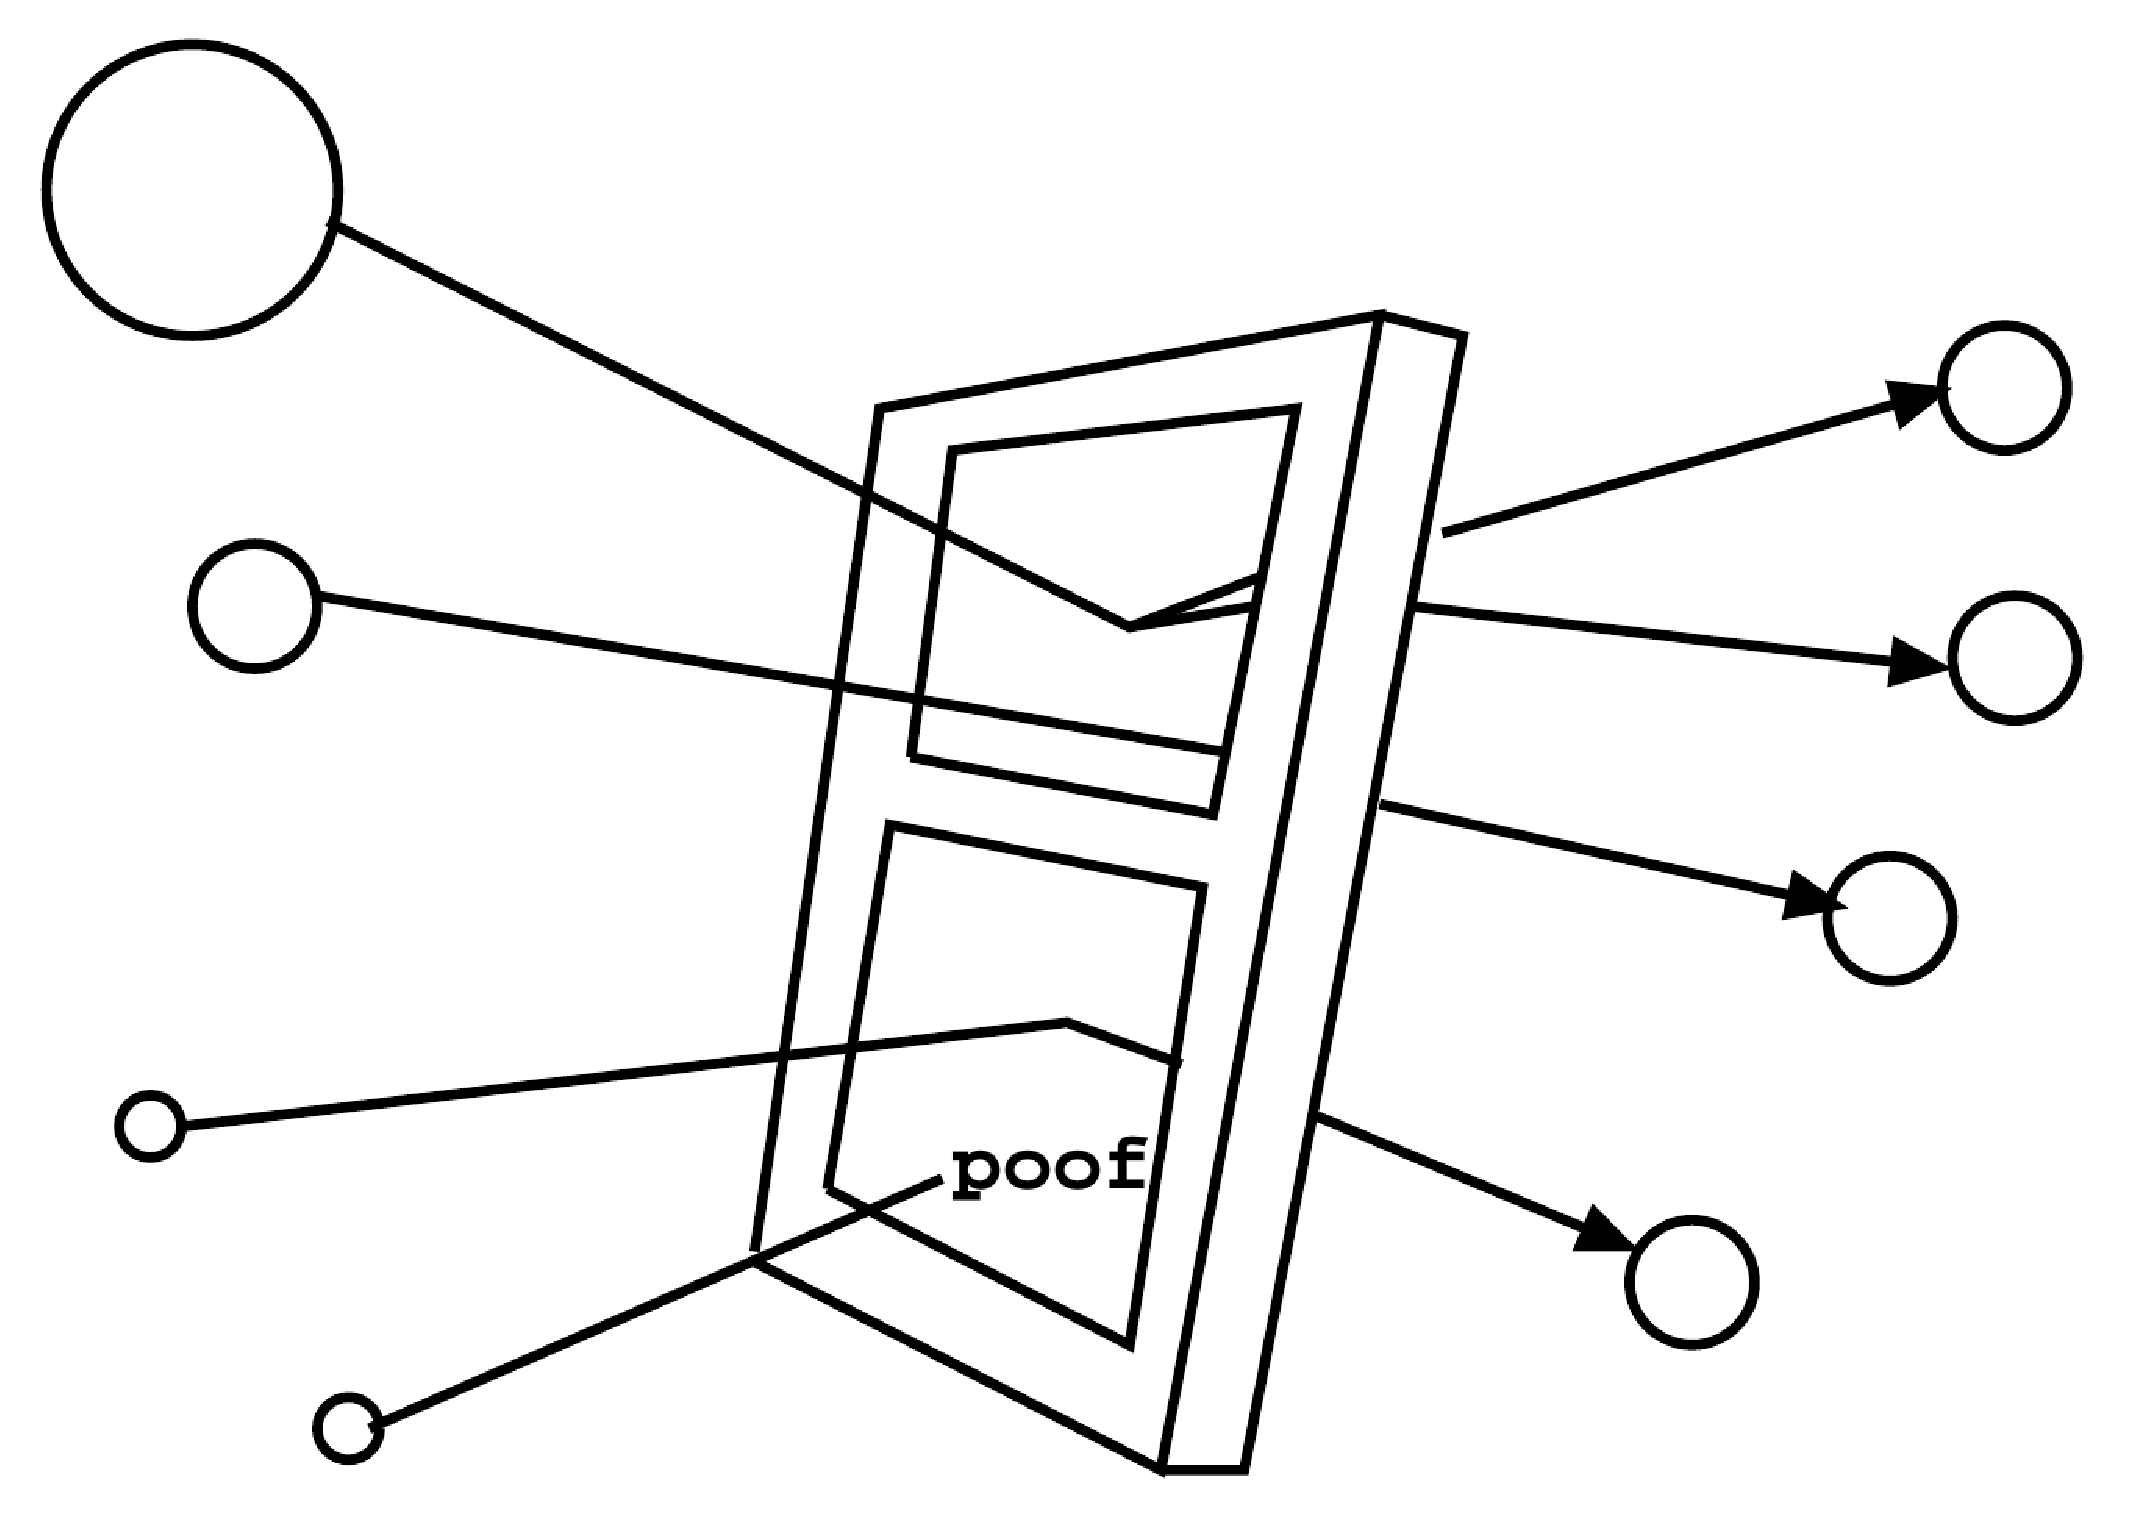
\includegraphics[width=0.85\textwidth]{img/ww-mcnp.eps}
\caption{Weight window phase space splitting and Russian roulette \cite{mcnp}.}
\label{fig:ww}
\end{figure}

The weight window may be used alone to good effect, but it is particularly powerful
when used in conjunction with other variance reduction techniques that introduce large
variations in particle weight. Well-specified weight windows keep the Monte Carlo 
solution from severe perturbations resulting from high-weight particles and 
simultaneously keep computational resources from wasting time on low-weight particles
by rouletting them.

\paragraph{Modified Sampling Methods}\mbox{} \\

Modified sampling methods alter the statistical sampling of a problem to increase the 
number of tallies per particle. For a given Monte Carlo event, it is possible to 
sample from an arbitrary distribution rather than the physical probability as long as 
the particle weights are adjusted to compensate. With modified sampling methods, 
sampling is done from distributions that send particles in desired directions or into 
other desired regions of phase space such as time or energy. Modified sampling methods
may also change the location or type of collisions. Categories of modified sampling
methods include implicit capture, forced collisions, and source biasing.

Using implicit capture (also called implicit absorption or survival biasing), 
particles are never killed by absorption. Instead, a particle's weight is reduced by
the absorption probability at each collision, allowing important particles to
survive by not being lost to absorption. Implicit capture can be thought of as a 
splitting process in which a particle of weight $w_0$ is split into two particles: one
of weight $w_0(1-\frac{\Sigma_a}{\Sigma_t})$ that survives and is 
subsequently followed, and one of weight $w_0\frac{\Sigma_a}{\Sigma_t}$ that is
instantaneously killed \cite{mcnp}.

The forced collision method increases sampling of collisions in specified spatial 
cells. Particles undergoing forced collisions are split into collided and uncollided
parts. The collided part of the particle is forced to react within the current cell,
while the uncollided part of the particle exits the cell without collision. When the
track of the uncollided particle portion is continued, it is followed with weight
$w_0e^{-\Sigma_t d}$, where $w_0$ is the original particle weight and $d$ is the
distance traveled between the splitting site and the cell boundary. The collided part
of the particle thus reacts with weight $w_0\left(1 - e^{-\Sigma_t d}\right)$. These
resultant weights are chosen to reflect the actual physics of the problem; 
$e^{-\Sigma_t d}$ is the probability of exiting the cell without collision, and 
$1 - e^{-\Sigma_t d}$ is the probability of colliding in the cell. One of these two
things must happen to the original particle of weight $w_0$, so we observe that the starting
weight is preserved.

Finally, particle sources may be biased with respect to one or more variables. This
allows for greater numbers of particles to be produced in more important ranges of 
each biased variable, with the particles' weights reduced accordingly. In the relevant
example of the neutron shielding problem, one may start more particles
at high energies and in strategic directions in order to get more particles to 
contribute to the desired solution. The corresponding weights of the particles are 
altered to correct the statistical distribution.

\subsection{Deterministic Methods}

In the case of deterministic methods, each of the six independent variables of the 
steady-state NTE is discretized, relevant boundary conditions are imposed, and the 
resulting system of linear algebraic equations is iterated over until an acceptable
solution has been reached. We limit the discussion here to the discretization of the
integro-differential form of the NTE and the finite-volume discrete ordinates method.

These discretizations introduce some errors into the calculations, with the
discretization of some variables being more problematic than others. For example, it
is functionally straightforward to discretize the energy and spatial variables, 
while discretizing angular space using the discrete ordinates method is more mathematically
intricate and often brings deleterious errors (``ray effects'') into problem solutions.
Deterministic methods may converge more quickly than Monte Carlo methods, especially
in the case of shielding problems, though the solutions are often plagued by the
aforementioned inaccuracies.

\subsubsection{Discretization of the Neutron Transport Equation}
\label{sec:disc}

\paragraph{Energy Discretization - The Multigroup Approximation}\mbox{} \\

Discretization of the energy variable is known as the ``multigroup'' approximation; 
it is relatively straightforward from a mathematical standpoint. Energy is broken up into $G$ 
groups, where the $g^{th}$ group has an upper bound of energy
$E_g$ and a lower bound of energy $E_{g+1}$ as shown in Figure \ref{egrid}. The highest energy 
group has $g = 0$ and the lowest energy group has $g = G-1$. This convention is used because 
neutrons are generally born at higher energies (starting in group 0 or 1) and scatter down to 
lower energies before undergoing an absorption reaction.

\begin{figure}[!thb]
\centering
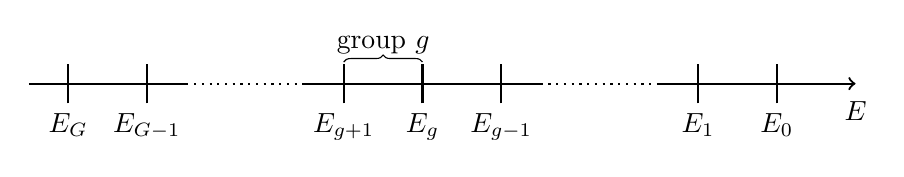
\begin{tikzpicture}
\draw[thick] (-5,0) -- (-3,0);
\draw[thick,dotted] (-3,0) -- (-1.5,0);
\draw[thick] (-1.5,0) -- (1.5,0);
\draw[thick,dotted] (1.5,0) -- (3,0);
\draw[thick,->] (3,0) -- (5.5,0);
\draw[thick] (-4.5,-0.25)--(-4.5,0.25);
\node [below] at (-4.5,-0.25) {$E_G$};
\draw[thick] (-3.5,-0.25)--(-3.5,0.25);
\node [below] at (-3.5,-0.25) {$E_{G-1}$};
\draw[thick] (-1,-0.25)--(-1,0.25);
\node [below] at (-1,-0.25) {$E_{g+1}$};
\draw[thick] (0,-0.25)--(0,0.25);
\node [below] at (0,-0.25) {$E_{g}$};
\node[above] at (-0.5, 0.25) {group $g$};
\draw[decorate,decoration={brace}](-1,0.275) -- (0,0.275);
\draw[thick] (1,-0.25)--(1,0.25);
\node [below] at (1,-0.25) {$E_{g-1}$};
\draw[thick] (3.5,-0.25)--(3.5,0.25);
\node [below] at (3.5,-0.25) {$E_1$};
\draw[thick] (4.5,-0.25)--(4.5,0.25);
\node [below] at (4.5,-0.25) {$E_0$};
\node [below] at (5.5,-0.1) {$E$};
\end{tikzpicture}
\caption{Discretized energy grid.}
\label{egrid}
\end{figure}

\FloatBarrier
Discretizing the NTE with respect to energy on this grid gives the $G$ multigroup
equations

\noindent\begin{minipage}{0.7\textwidth}
\begin{multline*}
\label{eq:mg_nte}
\bo \cdot \nabla \psi^g(\vecr,\bo) + \Sigma_t^g(\vecr) \psi^g(\vecr,\bo) =  \\
\sum_{g'=0}^{G-1}\int_{4\pi} \Sigma_s^{g'\rightarrow g}(\vecr,\bo'\cdot\bo)
\psi^{g'}(\vecr,\bo')d\bo' + Q^g(\vecr,\bo),
\end{multline*}
\end{minipage}
\hspace{-0.5cm}
\begin{minipage}{0.3\textwidth}
\begin{align}
\begin{split}
g &= 0,1,\ldots,G-1.
\end{split}
\end{align}
\end{minipage}
\vspace{0.1cm}

\noindent Here it is assumed that, within each energy group, the angular flux may be
approximated as the product of some known function of energy $f(E)$ and the group flux
$\psi^g(\vecr, \bo)$ as

\begin{equation}
\psi(\vecr,E,\bo) \approx f(E)\psi^g(\vecr,\bo), \quad E_{g+1} < E \leq E_{g}\:,
\end{equation}

\noindent where $f(E)$ is normalized such that $\int_{E_g+1}^{E_{g}}f(E)dE = 1$. With 
this, the multigroup cross sections and the group source are similarly defined
\cite{lm} as

\begin{align}
\Sigma_t^g(\vecr) &= \int_{E_{g+1}}^{E_{g}}\Sigma_t(\vecr,E)f(E)dE, \\
\Sigma_s^{g'\rightarrow g}(\vecr,\bo'\cdot\bo) &= \int_{E_{g+1}}^{E_{g}}\int_{E_{g'+1}}^{E_{g'}}
\Sigma_s(\vecr, E'\rightarrow E, \bo'\cdot\bo)f(E')dE'dE, \\
Q^g(\vecr,\bo) &= \int_{E_{g+1}}^{E_{g}}Q(\vecr,E,\bo)dE.
\end{align}

\paragraph{Spatial Discretization}\mbox{} \\

In the interest of completeness, we will briefly discuss the discretization of space.
The LDO equations are inherently three-dimensional \cite{ahrens}, so we will restrict
the discussion to three-dimensional space with point positions specified by Cartesian
coordinates. A general mesh cell is shown in Figure \ref{fig:spatial_mesh}.

\begin{figure}[!htb]
\centering
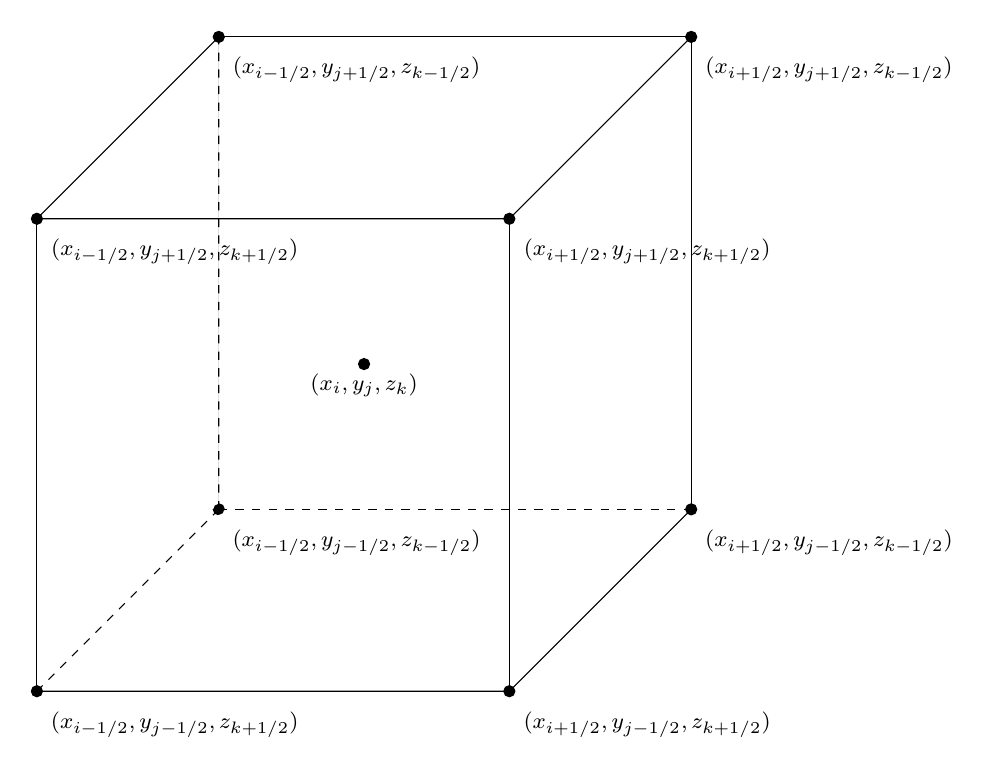
\begin{tikzpicture}
\filldraw (xyz cs:x=-3,y=-3,z=3) circle (2pt) node {} -- 
          (xyz cs:x=3,y=-3,z=3) circle (2pt) node {};
\node[fill,circle,inner sep=0pt, minimum size = 2pt,
      label={[shift={(1.75,-0.75)}]
      \footnotesize$(x_{i-1/2}, y_{j-1/2}, z_{k+1/2})$}] 
      at (xyz cs:x=-3,y=-3,z=3) {};
\node[fill,circle,inner sep=0pt, minimum size = 2pt,
      label={[shift={(1.75,-0.75)}]
      \footnotesize$(x_{i+1/2}, y_{j-1/2}, z_{k+1/2})$}] 
      at (xyz cs:x=3,y=-3,z=3) {};
\filldraw (xyz cs:x=-3,y=3,z=3) circle (2pt) node {} -- 
          (xyz cs:x=3,y=3,z=3) circle (2pt) node {};
\node[fill,circle,inner sep=0pt, minimum size = 2pt,
      label={[shift={(1.75,-0.75)}]
      \footnotesize$(x_{i-1/2}, y_{j+1/2}, z_{k+1/2})$}] 
      at (xyz cs:x=-3,y=3,z=3) {};
\node[fill,circle,inner sep=0pt, minimum size = 2pt,
      label={[shift={(1.75,-0.75)}]
      \footnotesize$(x_{i+1/2}, y_{j+1/2}, z_{k+1/2})$}] 
      at (xyz cs:x=3,y=3,z=3) {};
\filldraw (xyz cs:x=-3,y=3,z=3) -- 
          (xyz cs:x=-3,y=3,z=-3) circle (2pt) node[] {};
\node[fill,circle,inner sep=0pt, minimum size = 2pt,
      label={[shift={(1.75,-0.75)}]
      \footnotesize$(x_{i-1/2}, y_{j+1/2}, z_{k-1/2})$}] 
      at (xyz cs:x=-3,y=3,z=-3) {};
\filldraw (xyz cs:x=3,y=3,z=3)  -- 
          (xyz cs:x=3,y=3,z=-3) circle (2pt) node {};
\node[fill,circle,inner sep=0pt, minimum size = 2pt,
      label={[shift={(1.75,-0.75)}]
      \footnotesize$(x_{i+1/2}, y_{j+1/2}, z_{k-1/2})$}] 
      at (xyz cs:x=3,y=3,z=-3) {};
\filldraw (xyz cs:x=3,y=-3,z=3) -- 
          (xyz cs:x=3,y=-3,z=-3) circle (2pt) node {};
\node[fill,circle,inner sep=0pt, minimum size = 2pt,
      label={[shift={(1.75,-0.75)}]
      \footnotesize$(x_{i+1/2}, y_{j-1/2}, z_{k-1/2})$}]
      at (xyz cs:x=3,y=-3,z=-3) {};
\draw (xyz cs:x=-3,y=-3,z=3) -- (xyz cs:x=-3,y=3,z=3);
\draw (xyz cs:x=3,y=-3,z=3) -- (xyz cs:x=3,y=3,z=3);
\draw (xyz cs:x=-3,y=3,z=-3) -- (xyz cs:x=3,y=3,z=-3);
\draw (xyz cs:x=3,y=-3,z=-3) -- (xyz cs:x=3,y=3,z=-3);
\node[fill,circle,inner sep=0pt, minimum size = 2pt,
      label={[shift={(1.75,-0.75)}]
      \footnotesize$(x_{i-1/2}, y_{j-1/2}, z_{k-1/2})$}] 
      at (xyz cs:x=-3,y=-3,z=-3) {};
\filldraw[dashed] (xyz cs:x=-3,y=-3,z=-3) circle (2pt) node {} -- 
                  (xyz cs:x=-3,y=3,z=-3);
\draw[dashed] (xyz cs:x=-3,y=-3,z=-3) -- (xyz cs:x=3,y=-3,z=-3);
\draw[dashed] (xyz cs:x=-3,y=-3,z=-3) -- (xyz cs:x=-3,y=-3,z=3);
\filldraw (xyz cs: x=0,y=0,z=0) circle (2pt) node[below] 
          {\footnotesize$(x_i, y_j, z_k)$};
\end{tikzpicture}
\caption{General three-dimensional mesh cell \cite{exmm}.}
\label{fig:spatial_mesh}
\end{figure}

The mesh cell is centered at the $i^{th}$ position along the $x$-axis, the $j^{th}$
position along the $y$-axis, and the  $k^{th}$ position along the $z$-axis. Indexing
is such that there are $I$ mesh cells with $I+1$ grid points in the $x$-direction, $J$ mesh
cells with $J+1$ grid points in the $y$-direction, and $K$ mesh cells with $K+1$ grid points in 
the $z$-direction. It is assumed that all material 
properties are constant within a given cell. In order to eventually solve for the 
scalar flux in a given system, we are interested in solving for the angular flux at 
the center of each mesh cell, resulting in the $G\times I \times J \times K$
equations shown in Equation \ref{eq:mg_xyz_nte}.

\begin{minipage}{0.65\textwidth}
\begin{multline*}
\label{eq:mg_xyz_nte}
\bo\cdot\nabla\psi^g_{i,j,k}(\bo)+\Sigma_{t,i,j,k}^g\psi^g_{i,j,k}(\bo) =  \\
\sum_{g'=0}^{G-1}\int_{4\pi} \Sigma_{s,i,j,k}^{g'\rightarrow g}(\bo'\cdot\bo)
\psi^{g'}_{i,j,k}(\bo')d\bo' + Q^g_{i,j,k}(\bo),
\end{multline*}
\end{minipage}
\begin{minipage}{0.31\textwidth}
\begin{align}
\begin{split}
g &= 0,1,\ldots,G-1,\\
i &= 1,2,\ldots,I,\\
j &= 1,2,\ldots,J,\\
k &= 1,2,\ldots,K.
\end{split}
\end{align}
\end{minipage} \strut

\noindent To solve for these cell-centered flux 
quantities in practice, auxiliary equations are introduced. As these are specific to the 
spatial discretization employed in a given solution and do not differ between the classical
discrete ordinates equations and the LDO formulation, we refer the reader to Reference
\cite{denovo} for more detail on spatial differencing and solution methods.

\paragraph{Angular Discretization - Discrete Ordinates}\mbox{} \\
\label{sec:do}

The last part of phase space to discretize in the time-independent NTE is angle.
The discrete ordinates method is the most common angular discretization method
incorporated into general-purpose neutron transport codes \cite{lm}. It is a 
collocation method that requires the solution of the NTE to be exact at a 
distinct number of angles $\bo_n$:

\noindent\begin{minipage}{0.69\textwidth}
\begin{align*}
\bo_n&\cdot\nabla\psi^{g,n}_{i,j,k}+\Sigma_{t,i,j,k}^g\psi^{g,n}_{i,j,k} = \\
&\sum_{g'=0}^{G-1}\sum_{\ell=0}^P \Sigma_{s,\ell,i,j,k}^{g'\rightarrow g}
\bigg[\Ye{\ell 0}{n}\phi_{\ell 0}^{g'} + \sum_{m=1}^{\ell}
\bigg(\Ye{\ell m}{n}\phi_{\ell m}^{g'} \\
&\qquad\qquad\qquad\qquad\qquad\qquad
 + \Yo{\ell m}{n}\vartheta_{\ell m}^{g'}\bigg)\bigg]
 + Q^{g,n}_{i,j,k},
\end{align*}
\end{minipage}
\hspace{-0.55cm}
\begin{minipage}{0.31\textwidth}
\begin{align}
\begin{split}
g &= 0,1,\ldots,G-1,\\
i &= 1,2,\ldots,I,\\
j &= 1,2,\ldots,J,\\
k &= 1,2,\ldots,K,\\
n &= 1,2,\ldots,N.
\label{eq:do}
\end{split}
\end{align}
\end{minipage}
\vspace{0.1cm}

\noindent Here, $\psi^n \equiv \psi(\bo_n)$ and the angles are integrated by a
quadrature rule such that their corresponding weights $w_n$ sum to $4\pi$. Weights and
ordinates (``quadrature sets'') are chosen in such a way as to provide good 
approximations to angular integrals used to evaluate scalar flux \cite{lm,exmm}. The 
upper limit of summation for the scattering term spherical harmonic expansion, denoted
as $P$ in Equation \ref{eq:do}, is known as the ``\pn order''. The scattering cross section
coefficient values $\Sigma_{s,\ell,i,j,k}^{g'\rightarrow g}$ come from data libraries based on
experimental measurements.

The scattering source is expanded in terms of spherical harmonics:

\begin{equation}
\phi_{\ell,i,j,k}^{g}=\sum_{n=1}^N \Ye{\ell m}{n}w_n\psi^{g,n}_{i,j,k}\ \text{ and }\
\vartheta_{\ell,i,j,k}^{g} = \sum_{n=1}^N \Yo{\ell m}{n}w_n\psi^{g,n}_{i,j,k},
\label{sph_harm_exp}
\end{equation}

\noindent where $\phi$ and $\vartheta$ are
referred to as the ``flux moments''. 
Here, $\Ye{\ell m}{n}$ and $\Yo{\ell m}{n}$ are the ``even'' and ``odd'' 
real components of the spherical harmonic functions, defined as \cite{exmm}

\begin{equation}
\Ye{\ell m}{n} = (-1)^m\sqrt{(2-\delta_{m0})\frac{2\ell+1}{4\pi}
                       \frac{(\ell-m)!}{(\ell+m)!}}
                       P_{\ell m}(\cos\theta)\cos(m\varphi),
\label{eq:sph_e}
\end{equation}
\begin{equation}
\Yo{\ell m}{n} = (-1)^m\sqrt{(2-\delta_{m0})\frac{2\ell+1}{4\pi}
                       \frac{(\ell-m)!}{(\ell+m)!}}
                       P_{\ell m}(\cos\theta)\sin(m\varphi).
\label{eq:sph_o}
\end{equation}

\noindent In Equations \ref{eq:sph_e} and \ref{eq:sph_o}, $P_{\ell m}(\cos\theta)$ is 
the associated Legendre polynomial and $(\theta,\varphi)$ are the components of $\bo$ 
as shown in Figure \ref{fig:ang} and Equations \ref{eq:ang_disc} -- \ref{eq:ang_sum}. It is
assumed that the double differential scattering cross section depends only on the dot product of
the incoming and outgoing angles of the particle undergoing scattering.

To summarize Equations 
\ref{eq:do} -- \ref{eq:sph_o}, we note that the double differential scattering cross section is
expanded into the real components of the spherical harmonic functions, which can be represented
with Legendre polynomials; these are then multiplied with the angular flux moments expanded into
spherical harmonic functions.

\begin{figure}[!hbt]
\begin{minipage}{0.5\textwidth}
\begin{tikzpicture}
\coordinate (origin) at (0,0,0);
\coordinate (omega) at (2,4,7);
\coordinate (xaxis) at (0,0,9);
\coordinate (yaxis) at (3,0,0);
\coordinate (diag) at (2,5,0);
% axes
\draw[thick,->] (xyz cs:x=0) -- (xyz cs:x=3) node[right] {$x$};
\draw[thick,->] (xyz cs:y=0) -- (xyz cs:y=5) node[above] {$y$};
\draw[thick,->] (xyz cs:z=0) -- (xyz cs:z=8) node[below] {$z$};
% dashed box lines
\draw[dashed] (xyz cs:z=7,y=4) -- (xyz cs:z=7,y=0.25) node[left] {$\xi$};
\draw[dashed] (xyz cs:z=7,y=0) -- (xyz cs:z=7,x=2);
\draw[dashed] (xyz cs:z=7,x=2) -- (xyz cs:z=7,y=4,x=2);
\draw[dashed] (xyz cs:z=7,y=4,x=0) -- (xyz cs:z=7,y=4,x=2);

\draw[dashed] (xyz cs:x=2,z=0) -- (xyz cs:x=2,z=7);
\draw[dashed] (xyz cs:x=2,z=0,y=4) -- (xyz cs:x=2,z=0); 
\draw[] (xyz cs:x=2.3,y=-0.1,z=0) -- (xyz cs:x=2.3,y=-0.1,z=0) node[above] {$\mu$};
\draw[dashed] (xyz cs:x=2,z=0,y=4) -- (xyz cs:x=0,z=0,y=4) node[left] {$\eta$}; 
\draw[dashed] (xyz cs:x=0,z=0,y=4) -- (xyz cs:z=7,y=4);
\draw[dashed] (xyz cs:x=2,z=0,y=4) -- (xyz cs:z=7,y=4,x=2);

\draw[thick,->] (xyz cs:x=0,y=0,z=0) -- (xyz cs:x=2,z=7,y=4);
\draw[] (xyz cs:x=2,z=7,y=4) -- (xyz cs:x=2,z=7,y=4) node[above] {$\bo$};
\draw[dashed] (xyz cs:x=2,z=0,y=4) -- (xyz cs:x=0,z=0);
\draw[dashed] (xyz cs:z=7,y=0) -- (xyz cs:x=2,z=7,y=4);

\pic [draw,<-,angle radius=0.3cm,angle eccentricity=1.4,"$\theta$"]
     {angle = omega--origin--xaxis};
\pic [draw,->,angle radius=0.5cm,angle eccentricity=1.4,"$\varphi$"]
     {angle = yaxis--origin--diag};
\end{tikzpicture}
\caption{Angular coordinate system \cite{exmm}.}
\label{fig:ang}
\end{minipage}
\begin{minipage}{0.5\textwidth}
\begin{subequations}
\begin{align}
\label{eq:ang_disc}
&\xi = \cos\theta \\
&\mu = \sqrt{1-\xi^2}\cos\varphi \\
&\eta = \sqrt{1-\xi^2}\sin\varphi
\end{align}
\end{subequations}
\begin{equation}
\label{eq:ang_sum}
\mu^2 + \eta^2 + \xi^2 = 1
\end{equation}
\end{minipage}
\end{figure}

\FloatBarrier Commonly-used quadrature sets include level-symmetric, Gauss-
Legendre product, quadruple range (QR) product, and linear-discontinuous
finite element (LDFE). The various quadrature set types have different
properties with each being better for certain classes of problems. For
example, relatively coarse (sixteen angles per octant) QR product quadratures
are generally sufficient for generating variance reduction parameters for
neutron transport problems, but more finely resolved quadrature sets are
recommended for photon transport problems \cite{advantg}. Level-symmetric
quadrature sets are widely applied for general applications \cite{lm} but
tend to exhibit far more ray effects than QR product quadratures
\cite{advantg}. In the following subsection, we will discuss ray effects in
greater detail.

\subsubsection{Ray Effects}
\label{sec:ray}

Ray effects are unphysical computational anomalies in the scalar flux solution that 
arise from the discrete ordinates formulation. Because the NTE is only evaluated  
 at a finite number of discrete angles, the number of directions in 
which particles may stream is restricted. As a consequence of this, contributions to 
the scalar flux from uncollided particles are limited to those from the discrete 
angles along which particle sources are ``visible'' \cite{lathrop}. A demonstrative
example of ray effects is shown in Figure \ref{fig:ray}. The plot shows results from 
the PARTISN \cite{partisn} code using a triangular $P_n - T_n$ quadrature with
48 points and a
scattering ratio of $c = 0.25$ \cite{ahrens}. Although the point source
emits neutrons isotropically, the scalar flux calculated at a given radius out from 
the source sees contributions only from the discrete angles along which particles may
stream. That is, the flux at a given distance from the point source is actually equal 
in all directions and so the figure should appear to be a sphere, but the discrete
angles restrict streaming pathways to the rays shown in the image. 

\begin{figure}[!htb]
\centering
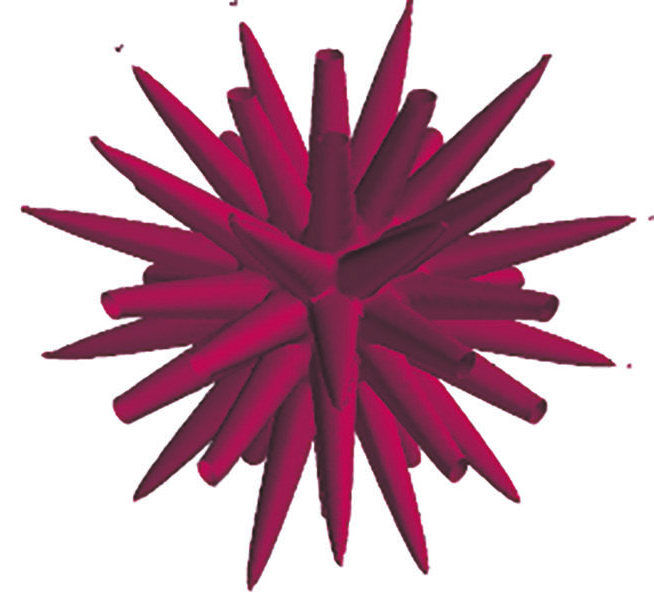
\includegraphics[width=0.5\textwidth]{img/ray-effects.png}
\caption{Isosurface plot of scalar flux from a point source \cite{ahrens}.}
\label{fig:ray}
\end{figure}

The severity of ray effects in a given simulation depends on the properties of
the  sources. The largest consequences tend to occur in scenarios with localized
sources and relatively minimal scattering. When using the discrete ordinates
approximation in a purely absorbing medium, regardless of the accuracy of the
angular flux calculations and the number of discrete angles used, it is always
possible to get far enough away from a localized source such that a poor value
of the scalar flux is obtained at that point \cite{lathrop}. In a scattering
medium with localized sources, angular flux values are incorrect because they
depend  on integrals that are poorly approximated by the quadrature formulation.
In contrast  to this, neutrons exiting scattering reactions are generally less
localized and  consequently tend to  mitigate ray effects. As we will see later
in the chapter, one key point of interest in using the LDO equations as part of
a hybrid method calculation is that the LDO equations mitigate ray effects when
higher-order quadrature sets are used  \cite{ahrens}.

\subsection{Hybrid Methods}

Hybrid methods aim to combine the previously described Monte Carlo
methods and deterministic methods in such a way as to perform calculations that result
in statistically meaningful results within a tractable period of computation time.
Generally, these hybrid methods are implemented such that the solution(s) from a 
deterministic code are used to inform a Monte Carlo code. When this is done well, the
Monte Carlo code converges more quickly than without the information from the
deterministic solution(s).

Specifically, an adjoint and/or forward flux solution generated by a deterministic 
transport solver is used to make a weight window map for a Monte Carlo run. As was
noted earlier, weight windows are most effective when specified well and when used in
conjunction with other variance reduction techniques. Because developing effective
weight window maps can be labor-intensive and require a user to have significant 
\textit{a priori} knowledge about the problem being solved, automated hybrid methods
have been developed to couple deterministic solutions to Monte Carlo transport
calculations.

\section{Previous Work}

Substantial effort has been placed into the development and automated execution of
hybrid methods. This section will discuss previous work in this field with a 
particular emphasis on the present state of hybrid methods as well as hybrid methods 
that incorporate neutron direction of travel.

Here we begin by describing the CADIS (consistent adjoint driven importance sampling)
and \fwc\ (forward-weighted consistent adjoint driven importance sampling) methods, 
which are the current state
of the art of Monte Carlo variance reduction parameter generation. These are 
introduced first because, as will be described in more detail later, this work 
employs solutions of the LDO equations in combination with the CADIS and \fwc\ 
methods via the ADVANTG software. Following this, we present a discussion of selected 
work in angle-informed hybrid methods, focusing on variants of CADIS and \fwc.

\subsection{CADIS and FW-CADIS}

\subsubsection{CADIS}
\label{sec:cadis}

The CADIS method was introduced by Wagner and Haghighat in 1997 to automate Monte 
Carlo variance reduction parameter generation \cite{cadis}. CADIS is based on the 
source biasing and weight window techniques described above, does not depend heavily 
on user experience, and was implemented as described in Reference \cite{cadis} in the 
MCNP \cite{mcnp} code. Most importantly, the CADIS method produces source biasing 
parameters and weight window target values such that particles are born with the target
weights. Since CADIS is used heavily in this work, it is pertinent to 
describe the theory behind the method.

The goal of most Monte Carlo neutron transport problems is to calculate some response
(scalar flux, dose, etc.) at some location in phase-space. This can be posed as 
solving the following integral equation:

\begin{equation}
R = \int_P \psi(P)\sigma_d(P)dP,
\label{eq:cadis_r1}
\end{equation}

\noindent where $R$ is the response of interest, $\psi$ is the neutron angular flux,
and $\sigma_d$ is some objective function in the phase-space $(\vecr, E, \bo) \in P$.
We now introduce the adjoint identity

\begin{equation} 
\langle \psi^{\dagger}, H\psi\rangle=\langle\psi , H^{\dagger}\psi^{\dagger}\rangle
\label{eq:adj}
\end{equation}

\noindent where $H$ is the transport operator and the dagger superscript indicates an 
adjoint quantity. Using Equation \ref{eq:adj} and some algebraic manipulations, it 
can be shown that

\begin{equation}
R = \int_P \psi^{\dagger}(P)q(P)dP,
\label{eq:cadis_r2}
\end{equation}

\noindent where $\psi^{\dagger}$ and $q$ are the adjoint neutron angular flux function
and the particle source density, respectively. For a given problem with a vacuum 
boundary condition, Equations \ref{eq:cadis_r1} and \ref{eq:cadis_r2} are equivalent 
expressions for $R$. The adjoint neutron angular flux function $\psi^{\dagger}$ has 
physical meaning as the expected contribution to the response $R$ from a particle in 
phase-space $P$. In other words, the adjoint flux function is significant because it 
represents the importance of those source particles to the response of interest.

To calculate the response with the Monte Carlo method, the independent variables are
sampled from the probability density function (PDF) $q(P)$. However, this may not be
the best PDF from which to sample, so an alternative PDF $\qhat(P)$ can be introduced
into the integral:

\begin{equation}
R = \int_P \left[\frac{\psi^{\dagger}(P)q(P)}{\qhat(P)}\right]\qhat(P)dP,
\end{equation}

\noindent where $\qhat(P) \geq 0$ and the integral of $\qhat(P)$ over $P$ is 
normalized to unity. Then, the alternative PDF $\qhat(P)$ that will minimize the 
variance of the response is given by

\begin{equation}
\qhat(P) = \frac{\psi^{\dagger}(P)q(P)}{\int_P\psi^{\dagger}(P)q(P)dP}.
\label{eq:qhat}
\end{equation}

\noindent Looking at Equation \ref{eq:qhat}, we see that the numerator is the 
response from phase-space $P$ and the denominator is the total response $R$. Thus, 
this definition of $\qhat(P)$ is a measure of the contribution from phase-space $P$ 
to the response. It is useful to bias the sampling of source particles by this ratio 
of their contribution to the detector response.

Because the source variables are sampled from this new biased PDF, the statistical
weight of the source particles must be corrected such that

\begin{equation}
w(P)\qhat(P) = w_0q(P),
\label{eq:cadis_w1}
\end{equation}

\noindent where $w_0$ is the unbiased particle starting weight and is set equal to 1.
Substituting Equation \ref{eq:qhat} into Equation \ref{eq:cadis_w1} and solving for 
$w(P)$ gives the following expression for the statistical weight of the particles:

\begin{equation}
w(P) = \frac{\int_P\psi^{\dagger}(P)q(P)dP}{\psi^{\dagger}(P)}
= \frac{R}{\psi^{\dagger}(P)}.
\label{eq:cadis_w2}
\end{equation}

\noindent Equation \ref{eq:cadis_w2} demonstrates an inverse relationship between 
this adjoint (importance) function and the statistical particle weight. 

Now, let us consider the
transport process in this context. The integral transport equation for particle
density in the phase-space $P$ is given by

\begin{equation}
\psi(P) = \int K(P'\rightarrow P)\psi(P')dP' + q(P)
\label{eq:cadis_nte1}
\end{equation}

\noindent where $K(P'\rightarrow P)$ is the expected number of particles entering $dP$
about $P$ from an event in $P'$. Given the preceding discussion, we would like to 
transform Equation \ref{eq:cadis_nte1} to be in terms of the biased source 
distribution $\qhat(P)$. Defining

\begin{equation}
\psihat(P) = \frac{\psi(P)\psi^{\dagger}(P)}{\int \psi^{\dagger}(P)q(P)dP},
\end{equation}

\noindent we can write Equation \ref{eq:cadis_nte1} in terms of $\qhat(P)$ as

\begin{equation}
\psihat(P) = \frac{\psi^{\dagger}(P)}{\int \psi^{\dagger}(P)q(P)dP}
\int K(P'\rightarrow P)\psi(P')dP' + \qhat(P).
\label{eq:cadis_nte2}
\end{equation}

\noindent Equation \ref{eq:cadis_nte2} can also be written as

\begin{equation}
\psihat(P) = \int K(P'\rightarrow P)\psihat(P')
\left[\frac{\psi^{\dagger}(P)}{\psi^{\dagger}(P')}\right]dP' + \qhat(P)\:,
\end{equation}

\noindent which allows us to define

\begin{equation}
\khat(P' \rightarrow P) = K(P'\rightarrow P)
\left[\frac{\psi^{\dagger}(P)}{\psi^{\dagger}(P')}\right]
\end{equation}

\noindent and finally write

\begin{equation}
\psihat(P) = \int\khat(P' \rightarrow P)\psihat(P')dP' +\qhat(P).
\end{equation}

Because $K(P'\rightarrow P)$ is unknown, we simulate neutron transport in the usual
unbiased way and change the number of particles emerging in $P$ from an event in
$P'$ by the ratio of importances $\psi^{\dagger}(P)/\psi^{\dagger}(P')$. When this
ratio is above one, splitting occurs, and rouletting occurs when the ratio is less 
than one. The statistical weights of the particles resulting from splitting and/or
rouletting are then corrected such that

\begin{equation}
w(P)K(P' \rightarrow P)\left[\frac{\psi^{\dagger}(P)}{\psi^{\dagger}(P')}\right] = 
w(P')K(P' \rightarrow P)
\end{equation}

\noindent or

\begin{equation}
w(P) = w(P')\left[\frac{\psi^{\dagger}(P)}{\psi^{\dagger}(P')}\right].
\label{eq:cadis_w3}
\end{equation}

\noindent With this, reduced variance can be achieved when all source and transport
sampling is proportional to its importance. The source particles' energy and position
are sampled from the biased source distribution

\begin{equation}
\qhat(\vecr,E) = 
\frac{\phi^{\dagger}(\vecr,E)q(\vecr,E)}
{\int_V\int_E\phi^{\dagger}(\vecr,E)q(\vecr,E) dE\ d\vecr} 
= \frac{\phi^{\dagger}(\vecr,E)q(\vecr,E)}{R}.
\label{eq:cadis_sb}
\end{equation}

\noindent Here, the physical meaning of the numerator is the detector response from
space-energy element $(d\vecr,dE)$ and the denominator is the total detector response
$R$. As in the preceding derivation, this ratio is a measure of the particles' 
relative contribution to the detector response.

To bias particles undergoing the transport process, the weight window technique is 
applied. Weight window lower bounds $w_{\ell}$ must be calculated such that the
statistical weights defined in Equation \ref{eq:cadis_w2} fall at the center of the
weight window intervals. The width of a given interval is denoted by 
$c_u = w_u/w_{\ell}$, the ratio of upper and lower weight window values. The
weight window lower bounds are then given by

\begin{equation}
w_{\ell}(\vecr,E) = \frac{w}{\left(\frac{c_u +1}{2}\right)} 
= \frac{R}{\phi^{\dagger}(\vecr,E)}\frac{1}{\left(\frac{c_u +1}{2}\right)}.
\label{eq:cadis_tb}
\end{equation}

\noindent Using this definition, the weight window technique then performs particle
splitting and/or rouletting consistent with the statistical weight given in Equation
\ref{eq:cadis_w3}.

The key result of the foregoing discussion is that the statistical weights of the
source particles are within the bounds of the weight windows. In other words, the
source-biasing parameters and the weight window target values are consistent. This
circumvents the potential of particles being immediately split or rouletted upon birth
and avoids the resultant degradation in computational efficiency. We refer the reader
to Reference \cite{cadis} for a complete discussion of results and analysis of the initial
implementation of the CADIS method.

Note that Equations \ref{eq:cadis_sb} and \ref{eq:cadis_tb} use the scalar adjoint 
flux rather than the angular flux. This is consistent with the
original implementation of the CADIS method in MCNP as well as the implementation of
the method in ADVANTG; the scalar adjoint neutron flux function is used in both tools
\cite{cadis, advantg}. Historically, this was done to reduce the memory required for
the deterministic calculation as well as the weight window map. Additionally, the 
angular adjoint flux resulting from an \sn calculation was not considered to be 
sufficiently accurate due to the limited number of discrete angles used for the 
calculation. Further, people have
generally not developed weight windows that are a function of angle.

The CADIS method is very effective for automated optimization of localized detectors
but falls short of efficiently optimizing distributed responses. FW-CADIS, discussed 
in the next section, was developed to address this issue.

\subsubsection{FW-CADIS}
\label{sec:fwcadis}

FW-CADIS, introduced
by Wagner, Blakeman, and Peplow in 2009, is a variation on the CADIS method to 
increase the efficiency of Monte Carlo calculations of distributions and responses at 
multiple localized detectors \cite{fwcadis}.

For this global variance reduction method, a response with uniformly-low statistical 
uncertainty across all phase-space is desired. One way to target this for a given 
Monte Carlo simulation is to uniformly distribute the particles throughout the system.
Though this is not a physical response, it is a proxy for the goal of obtaining 
uniform uncertainty. It also indicates the possibility of developing an adjoint 
importance function that represents the importance of particles to achieving the goal
of uniform particle distribution.

With this new problem formulation, the problem of calculating particle density is cast
into the response formulation:

\begin{equation}
R = \int_{4\pi}\int_{V}\int_{E}\psi(\vecr,E,\bo)f(\vecr,E,\bo)dE\ dV\ d\bo,
\end{equation}

\noindent where $f(\vecr,E,\bo)$ is some function that converts angular neutron flux 
to Monte Carlo particle density. Recall that the angular neutron flux can be defined 
as the product of the physical particle density $n$ and velocity $v$:

\begin{equation}
\psi(\vecr,E,\bo) = n(\vecr,E,\bo)v(\vecr,E,\bo)
\label{eq:psi}
\end{equation}

\noindent and the physical particle density is related to the Monte Carlo particle 
density $m$ and the average particle weight $\bar{w}$ by

\begin{equation}
n(\vecr,E,\bo) = \bar{w}(\vecr,E,\bo)m(\vecr,E,\bo).
\label{eq:dens}
\end{equation}

\noindent Using Equations \ref{eq:psi} and \ref{eq:dens}, the Monte Carlo particle 
density can be estimated by

\begin{equation}
m(\vecr,E,\bo) = \frac{n(\vecr,E,\bo)}{\bar{w}(\vecr,E,\bo)} 
= \frac{\psi(\vecr,E,\bo)}{\bar{w}(\vecr,E,\bo)v(\vecr,E,\bo)}
\end{equation}

\noindent and the total Monte Carlo density can be estimated by

\begin{equation}
R = \int_{4\pi}\int_{V}\int_{E}\psi(\vecr,E,\bo)
\left[\frac{1}{\bar{w}(\vecr,E,\bo)v(\vecr,E,\bo)}\right]dE\ dV\ d\bo.
\label{eq:fwcadis_r}
\end{equation}

If the average particle weight is set proportional to the physical particle density,
then the Monte Carlo particle density should be approximately uniform in phase-space.
Substituting Equation \ref{eq:psi} into Equation \ref{eq:fwcadis_r} gives %eq 14

\begin{equation}
R = \int_{4\pi}\int_{V}\int_{E}\psi(\vecr,E,\bo)
\left[\frac{1}{\psi(\vecr,E,\bo)}\right]dE\ dV\ d\bo.
\end{equation}

\noindent By then defining the adjoint source as the bracketed term in the above
equation,

\begin{equation}
q^{\dagger}(\vecr,E,\bo) = \frac{1}{\psi(\vecr,E,\bo)},
\end{equation}

\noindent we can calculate an adjoint importance function that represents the
importance of particles to achieving the desired objective of uniformly distributed
Monte Carlo particles. This should, in turn, correspond to approximately uniform
statistical uncertainties. The method physically corresponds to weighting the adjoint
source with the inverse of the forward flux; the adjoint source will be high where the
forward flux is low and the adjoint source will be low where the forward flux is high.
With this method, after the adjoint has been determined, the standard CADIS procedures
are used to calculate consistent source biasing parameters and weight windows.

When considering implementation and use, it should be noted that, while the original
CADIS method requires only one deterministic calculation, the \fwc\ method requires
two (one forward and one adjoint) deterministic calculations. Additionally, like the
original CADIS method, \fwc\ is general and could be applied to all independent
variables of a problem, but the implementation has been limited to space and energy. 

\subsection{Directional CADIS}

Noting the marked performance of the CADIS and \fwc\ methods, their limited 
implementation in only space and energy, and the importance of particle direction, 
Peplow introduced directional CADIS in 2012 \cite{peplow}. Two versions of directional
CADIS were explored: one method that biases the source in space and energy while
preserving the original angular distribution of the particles, and one method that
biases the source in space, energy, and angle. Both new methods were tested against
standard CADIS for seven example problems, with the Monte Carlo FOM compared among the
methods for each problem.

Peplow notes that in many applications involving directionally dependent source 
distributions, the directional dependence is azimuthally symmetric about a given
reference direction $\mathbf{\hat{d}}$. With this, the angular distribution of the 
particles $q_i(\bo)$ can be expressed as the product of the uniform azimuthal 
distribution and a polar distribution about reference $\mathbf{\hat{d}}_i$. The 
angular particle distribution may then be written as 
$\frac{1}{2\pi}q_i(\bo\cdot\mathbf{\hat{d}}_i)$. Peplow also notes that the
geometric size of these directional sources tends to be small enough to allow each
source distribution to be expressed as the product of two separable distributions:
$q_i(\vecr,E,\bo) \approx q_i(\vecr, E)q_i(\bo)$.

The implementation of directional CADIS explored in this work was intended to
appropriately incorporate the importance of a particle traveling in a given direction
while also serving as a relatively simple modification of the standard CADIS method
that is less involved than a full treatment of space, energy, and angle. It starts 
with the approximation that the angular component of the adjoint flux 
$\psi^{\dagger}(\vecr,E,\bo)$ is separable and symmetric about the average adjoint
current direction $\hat{\mathbf{n}}(\vecr,E)$ such that

\begin{equation}
\psi^{\dagger}(\vecr,E,\bo) \approx
\phi^{\dagger}(\vecr,E)\frac{1}{2\pi}f(\bo\cdot\hat{\mathbf{n}}).
\end{equation}

\noindent From this, it is proposed that weight window targets can be developed that
are inversely proportional to the approximation of the adjoint angular flux:

\begin{equation}
\bar{w}(\vecr,E,\bo) = 
\frac{2\pi k}{\phi^{\dagger}(\vecr,E)f(\bo\cdot\hat{\mathbf{n}})}
\end{equation}

\noindent where $k$ is a constant of proportionality that is adjusted to make the
importance map consistent with the biased source(s). The implementation of the
following methods uses standard CADIS routines to compute the response per unit 
source $R$, the weight window target values $\bar{w}(\vecr,E)$, and the biased source 
$\hat{q}(\vecr,E)$ using only the adjoint scalar flux. The quantities are then
modified to include directional information.

\subsubsection{Without Directional Source Biasing}

Peplow asserts that the biased source $\hat{q}(\vecr,E,\bo)$ should be proportional
to both the true particle source distribution and the space-energy component of the
scalar adjoint flux:

\begin{equation}
\hat{q}(\vecr,E,\bo) = \frac{1}{R}
\left[q(\vecr,E)\frac{1}{2\pi}q(\bo\cdot\mathbf{\hat{d}})\right]
\phi^{\dagger}(\vecr,E),
\end{equation}

\noindent where the constant of proportionality $R$ is determined by forcing
$\hat{q}(\vecr,E,\bo)$ to be a PDF. Since the scalar adjoint flux is used here, the
directional distribution of the biased source is identical to that of the true source.
Detailed in Reference \cite{peplow}, the constant of proportionality $R$ is found to be equal to
the response per unit source from the traditional space-energy CADIS treatment. Thus,
the biased source can be expressed as

\begin{equation}
\hat{q}(\vecr,E,\bo) = \hat{q}(\vecr,E)\frac{1}{2\pi}q(\bo\cdot\mathbf{\hat{d}}). 
\end{equation}

The birth weight of a particle sampled from this distribution is independent of
direction and the proportionality constant $k$ for the target weight windows should be
chosen such that the weight window targets match the birth weight of the source
particles. This cannot be done generally because the particle birth weight is
independent of direction, but it can be done for a single point in phase space
$(\vecr_0,E_0,\bo_0)$ of the source such that

\begin{equation}
k = \frac{R}{2\pi}f\left(\bo_0\cdot\hat{\mathbf{n}}(\vecr_0,E_0)\right),
\end{equation}

\noindent where the average adjoint current direction $\hat{\mathbf{n}}(\vecr_0,E_0)$
is evaluated at the source location and energy and

\begin{equation}
\bar{w}(\vecr,E,\bo) = \bar{w}(\vecr,E)
\frac{f\left(\bo_0\cdot\hat{\mathbf{n}}(\vecr_0,E_0)\right)}
{f(\bo\cdot\hat{\mathbf{n}})}.
\end{equation}

\noindent Because the biased source and the weight window targets will match only at
the specified direction of interest $\bo_0$ at one specific position and energy, the
point $(\vecr_0,E_0,\bo_0)$ should be chosen carefully to represent the source
accurately and to minimize rouletting and/or splitting of particles just after birth.

It should be noted that this approach is exact for cases where no directional biasing
could be applied, e.g.\ monodirectional beam sources. Although the above discussion
considers only one particle source, this directional CADIS method may be extended to
multiple sources, as explained in detail in Reference \cite{peplow}.

\subsubsection{With Directional Source Biasing}

In this method, it is asserted that the biased source should be proportional
to both the true particle source distribution and the approximation of the angular
adjoint flux:

\begin{equation}
\hat{q}(\vecr,E,\bo) = \frac{1}{cR}
\left[q(\vecr,E)\frac{1}{2\pi}q(\bo\cdot\mathbf{\hat{d}}_i)\right]
\left[\phi^{\dagger}(\vecr,E)\frac{1}{2\pi}f(\bo\cdot\hat{\mathbf{n}}_0)\right],
\end{equation}

\noindent where the constant $cR$ is used to make $\hat{q}$ a PDF. Because the vector
$\hat{\mathbf{n}}_0$ is fixed over the source, the biased source is separable into
$\hat{q}(\vecr,E,\bo)=\hat{q}(\vecr,E)\hat{q}(\bo)$ where $\hat{q}(\bo)$ can be
further separated into the product of its azimuthal and polar distributions:

\begin{equation}
\hat{q}(\vecr,E,\bo) = 
\left[\frac{1}{R}q(\vecr,E)\phi^{\dagger}(\vecr,E)\right]
\left[\frac{1}{c}\frac{1}{4\pi^2}q(\bo\cdot\mathbf{\hat{d}})
f(\bo\cdot\hat{n}_0)\right].
\end{equation}

Both distributions $\hat{q}(\vecr,E)$ and $\hat{q}(\bo)$ are independent and each 
should be a PDF. For the space-energy distribution, the standard definition of $R$
still applies. For the angular distribution, the constant $c$ is found to be

\begin{equation}
c = \int\frac{1}{4\pi^2}q(\bo\cdot\hat{\mathbf{d}})f(\bo\cdot\hat{\mathbf{n}}_0)d\bo,
\end{equation}

\noindent which may be evaluated using numerical integration. It should be noted that
if either the original source directional distribution $q(\bo)$ or the adjoint
angular flux distribution at the source is isotropic, then $c$ reduces to a value of
$\frac{1}{4\pi}$.

Source particles sampled from the biased distribution are born with a starting weight
of

\begin{equation}
\bar{w}(\vecr,E,\bo) =
\frac{R}{\phi^{\dagger}(\vecr,E)}\frac{2\pi c}{f(\bo\cdot\hat{\mathbf{n}}_0)} = 
\bar{w}(\vecr,E)\frac{2\pi c}{f(\bo\cdot\hat{\mathbf{n}}_0)}\:,
\end{equation}

\noindent where the constant $k$ has been found to be equal to $cR$. As with the 
previously described method, the user selects one point $(\vecr_0,E_0,\bo_0)$ that is
representative of the entire source, where the biased source will match the target
weight windows. This method can also be extended to incorporate multiple sources.

\subsubsection{Results}

Sample problems of applications of interest were examined and compared between 
standard CADIS and directional CADIS. For most of these problems, directional CADIS 
outperformed standard CADIS, increasing the Monte Carlo FOM by a factor of around 2. Notable
cases in which directional CADIS performed more poorly than standard CADIS are a
neutron porosity tool problem and a gamma-ray litho-density tool problem with the
detector far away from the source. It should also be noted that, for a spherical boat
test problem with a source far away from the boat, both standard CADIS and directional
CADIS performed more poorly than an analog Monte Carlo calculation. For full details on the
test results, see Reference \cite{peplow}. In the conclusions of the report, Peplow 
notes that ``it is difficult to know \textit{a priori} which problems would benefit 
from the space/energy/angular treatments presented in this work more than from just 
using the standard space/energy CADIS.''

\subsection{CADIS-$\Omega$}

One of the most recent developments in the area of angle-informed hybrid methods is
\co, introduced by Munk et al.\ in 2016 \cite{cadisom}. This method calculates an
alternate form of the adjoint scalar flux quantity that is then used in the CADIS and
\fwc\ methods for generation of variance reduction parameters for local and global
response functions, respectively.

The alternative form of the adjoint scalar flux used in \co\ is defined as

\begin{equation}
\phi^{\dagger}_{\Omega}(\vecr,E) = 
\frac{\int_{4\pi} \psi(\vecr ,E,\bo)\psi^{\dagger}(\vecr,E,\bo)d\bo}
{\int_{4\pi}\psi(\vecr,E,\bo)d\bo}.
\end{equation}

\noindent Here, the product $\psi(\vecr ,E,\bo)\psi^{\dagger}(\vecr,E,\bo)$ is known
as the ``contributon flux''; contributons can be conceptualized as pseudo-particles
that carry ``response'' from a particle source to a detector. The contributon flux
incorporates information from both the forward particle flux as well as the adjoint
particle flux. It signifies the importance of a particle born from a forward source
moving towards an adjoint source. That is, when the contributon flux is used to 
generate an importance map, high importance will be assigned to particles that are
generated at the forward source and are likely to generate a response in the detector
(the adjoint source).

The \co\ method was implemented in the ADVANTG framework, with numerical experiments
performed testing variance reduction for problems run in MCNP5. Several
characterization problems with spatially-induced anisotropies were tested to
evaluate the new method when used with CADIS and \fwc. Here we will summarize the
problems tested and the results; a full discussion can be found in Reference 
\cite{munk}. Munk identified three categories of processes that affect particle flux 
anisotropy: strongly directional particle sources, strong differences between material
properties, and algorithmic limitations that result in ray effects.

Having grouped these processes, Munk tested a set of characterization problems, each
of which have different combinations of the above anisotropy-inducing mechanisms. Munk
also developed a set of metrics by which the anisotropy of the flux may be quantified
over the various problems. Similar to the conclusions drawn by Peplow, Munk found 
that it was difficult to predict for which problems \co\ should outperform CADIS. When
considering a parametric study of deterministic variables likely to affect angular 
flux (varying quadrature set order and \pn order) in a characteristic problem
composed of a steel beam embedded in concrete, \co\ achieved higher FOM values than 
standard CADIS for all quadrature and \pn orders at high energies. Similarly, for a
simple labyrinth geometry of an air maze through a concrete block, \co\ achieved lower
relative errors than did standard CADIS in the epithermal and fast neutron energy
groups.

\subsection{Other Notable Work}

Here we will briefly summarize other notable works in the area of angle-informed 
hybrid methods. We first introduce AVATAR, then discuss two following methods that
built off of the work.

\subsubsection{AVATAR}

AVATAR (Automatic Variance And Time of Analysis Reduction) was developed at Los Alamos
National Laboratory by Van Riper et al.\ in the 1990s to eliminate the need for
user-generated weight windows \cite{avatar}. The package may be thought of as a
predecessor to the various CADIS methods, as it constructs three-dimensional energy-
and angle-dependent weight windows for an MCNP run from an adjoint calculation using
the THREEDANT \cite{threedant} deterministic code.

The scalar adjoint fluxes resulting from THREEDANT are inverted by AVATAR to get the
lower weight window boundary in each mesh element of the problem. The weight windows
are then normalized such that source particles are born with weights inside of the
weight window. If angle-dependent weight windows are desired, the angular adjoint flux
is approximated using information theory \cite{avatar}; the full angular adjoint flux
was deemed to require an inordinate amount of storage at the time of development.

AVATAR's weight window mesh is independent of the Monte Carlo cells, so weight 
windows are applied at absolute particle positions rather than when particles pass
between weight window meshes. To protect against significant variance increases in
particle weight (and tally) due to large sampling distance, weight windows are applied
at a minimum of once per mean free path traveled by a particle.

AVATAR was tested on a model of a three-detector oil well logging tool consisting of
a gamma-ray source and three gadolinium detectors. The system was intended to
represent deep-penetration problems, as a small fraction of the gamma rays emitted
from the source actually reach the detectors. The detector nearest the gamma-ray
source has a collimator attached, adding an angular dependence to the tool modeled. 

Results from AVATAR were compared against MCNP's weight window generator (WWG). For
the three-detector problem described above, AVATAR's angle-dependent weight windows
delivered the highest FOM for the detector nearest the source as well as the 
``middle'' detector. The MCNP WWG delivered the highest FOM for
the detector furthest from the source, but it should be noted that the MCNP geometry
was hand-tuned for the WWG cases. When considering only a single detector, the
AVATAR angle-dependent weight windows outperformed the WWG for a detector near the
source as well as far from the source.

\subsubsection{Cooper and Larsen's Weight Windows}

Cooper and Larsen developed a method similar to FW-CADIS that uses weight windows to
distribute Monte Carlo particles uniformly throughout the system for the purpose of
efficiently solving global particle transport problems \cite{clww}. Rather than using
an adjoint deterministic solution for generation of weight windows, a forward solution
is used. The method presented employs solution of the forward quasi-diffusion 
equation, a modified diffusion equation that contains multiplicative correction terms
known as ``Eddington factors''.

The authors argue that a forward solution is more appropriate than an adjoint solution
in the context of automated weight window generation for Monte Carlo variance
reduction. This is supported by showing that if the center of the weight window in
each cell is chosen to be proportional to the density of the physical particles in the
cell, then the density of Monte Carlo particles throughout the system will be
approximately constant.

Cooper and Larsen construct ``isotropic'' weight windows as well as angle-dependent
weight windows, following the AVATAR method to formulate the latter. The authors note
that a uniform particle distribution in angle is not always optimal with respect to
computational efficiency, especially when considering problems with significant
streaming. It is the case that the angle-dependent weight windows developed in this 
work actually have the potential to reduce the FOM due to excessive Monte Carlo 
particle splitting in nonstreaming regions. To mitigate this by decreasing the amount 
of splitting incurred, the weight window experienced by particles traveling in 
directions opposite to the preferred direction is raised. This preserves the scalar 
flux, but not the current \cite{clww}.

Results are presented for two two-dimensional problems. In both problems, weight
windows were updated twice -- once after one-third of the histories had completed and
again after two-thirds of the particle histories had finished. The weight window
parameters were chosen to ensure a stable quasi-diffusion solution. The two problems
were chosen to rigorously test the global Monte Carlo method; the problems are
optically thick with scattering ratios sufficiently low such that the scalar flux
decreases by several orders of magnitude far away from the particle source. To 
observe the performance of the method on problems with significant angular effects,
the first problem includes a duct and the second problem includes a barrier.

For the problem including a duct, the Monte Carlo FOM values calculated in the 
individual spatial cells are vastly improved by the use of both weight window types
developed in this work. In particular, the solution estimates for the scalar flux are
very noisy far from the solution when only survival biasing is used. Additionally, the
angle-dependent weight window generates a slightly higher FOM in the duct region than
the isotropic weight window. Similarly, for the problem including a barrier, the use
of either type of weight window developed here results in a drastically more uniform
particle distribution. Again, the angular weight window outperformed the isotropic
weight window. Thus, from this work, we observe that incorporating angular
information into weight window generation can significantly improve Monte Carlo FOM
for problems with strong geometric anisotropies.

\subsubsection{LIFT}

LIFT, the local importance function transform, was introduced by Turner and Larsen in
1997 \cite{lift1, lift2} as a new automatic Monte Carlo variance reduction method that
closely approximates a zero-variance method through the use of biasing parameters. The
LIFT method is partially based on the exponential transform, which adjusts the 
distance to collision such that particles traveling toward the region of interest 
undergo fewer collisions than particles traveling away from the region of interest.
Particle weights are adjusted accordingly to keep the simulation unbiased. On top of
the conventional exponential transform, the LIFT method adds in energy and angular
biasing in each cell of the system.

LIFT uses scalar flux information from a deterministic adjoint solution to bias the
source distribution, distance to collision, scattering angle, and energy. The adjoint 
scalar flux is also used to formulate weight windows. In the implementation 
presented, the weight windows are not angle-dependent. The authors note that, in the 
LIFT implementation, the angle-dependent weight windows require the use of an 
analytic expression for the angular flux at every boundary and collision site and 
that this extra computational effort does not generally yield increased efficiency 
for the Monte Carlo calculation that then employs the angle-dependent weight windows.

The LIFT strategy can be summarized in two steps. First, an analytic function is
derived that is piecewise continuous in space and angle and approximates the adjoint
solution within each energy group and spatial cell of the Monte Carlo system. Then,
this approximate representation of the adjoint solution is used to transform the
original forward problem into a new problem that can be solved by a Monte Carlo 
simulation with reduced variance. Increased accuracy in the approximation of the
adjoint solution results in greater reduction of the variance, approaching zero
variance in the solution when using an exact representation. The authors note that 
this limit is unachievable and that the algebraic cost of obtaining and using more
accurate adjoint solutions must be balanced against the desired FOM. 

The authors compare LIFT against AVATAR, considered to be one of the most efficient
automated variance reduction techniques used in a major production code at the time of
publication. The overall result stated in Reference \cite{lift1} is that LIFT 
outperforms 
AVATAR in most problems. The reasons given for this are that LIFT particles have 
significantly shorter histories than AVATAR particles and that LIFT particles have
smaller weight fluctuations than AVATAR particles and thus require less splitting and 
Russian roulette. It is noted, however, that the two methods perform comparably for
problems where biasing is difficult (AVATAR does not use any biasing techniques other
than survival biasing, which LIFT also employs in addition to its other biasing).

It is seen that the LIFT method loses its advantage over survival biasing as the 
scattering ratio of a given problem approaches unity. While FOM values from LIFT
increase, the acceleration of the method compared to survival biasing becomes 
negligible \cite{lift1}. In Reference \cite{lift2}, numerical results and comparisons 
against
AVATAR are presented. We will briefly summarize the results and conclusions here,
focusing on results from the most complex scenario tested, as the work presented in 
this dissertation is concerned with three-dimensional multigroup problems.

Cooper and Larsen tested the LIFT method in combination with results from various
types of deterministic solutions as well as in combination with weight windows
generated from AVATAR. The most complex scenario tested was multigroup in energy 
and featured a concrete cube with a duct running through it. The duct was also
concrete but with a lower density than the bulk material; it had the source at one end,
the detector at the other end, and three bends along its path. In general, it was
found that incorporating angular information into the AVATAR and LIFT solutions 
improved the FOM for the Monte Carlo calculation when using either code \cite{lift2}.
Taking this result into consideration as well as other conclusions drawn in work 
discussed earlier in this chapter, we move forward onto discussing the LDO equations,
which will be developed and then used to incorporate angular information into Monte
Carlo variance reduction parameter generation.

\section{The Lagrange Discrete Ordinates (LDO) Equations}
\label{sec:ldo}

The Lagrange Discrete Ordinates (LDO) equations, shown in Equation \ref{eq:ldo}, are
formally the same as the classical discrete ordinates equations. The LDO equations
differ from the discrete ordinates equations in how the scattering source is 
calculated and in the representation of the angular flux. In this section, we give a
mathematical background for and a derivation of the LDO equations.

\subsection{Mathematical Background}
\label{sec:ldo_math}

Prior to deriving the LDO equations, it is useful to summarize relevant material from
approximation theory for functions defined on $\maths$, the unit sphere in 
$\mathbb{R}^3$. We start by denoting the space of square integrable functions on
$\maths$ as $L^2(\maths)$, where an orthonormal basis for $L^2(\maths)$ is given by 
the spherical harmonic functions

\begin{equation}
Y_{\ell}^m(\theta,\varphi) = (-1)^{\ell}
\sqrt{\frac{2\ell+1}{4\pi}\frac{(\ell-m)!}{(\ell+m)!}}
P_{\ell}^m(\cos\theta)e^{im\varphi}.
\end{equation}

\noindent Here, $\ell\geq 0$, $|m| \leq \ell$, $P_{\ell}^m$ is the associated 
Legendre function, and $\theta$ and $\varphi$ are the polar and azimuthal components 
of $\bo$, respectively. For a given positive integer $L > 0$, we define the 
rotationally invariant subspace of the spherical harmonics, $\hl$, as

\begin{equation}
\label{eq:span}
\hl = \text{span}\{Y_{\ell}^m: |m| \leq \ell, 0 \leq \ell \leq L\},
\end{equation}

\noindent with dimension $\dl = \dim\hl = (L+1)^2$. Said differently, $\hl$ is the 
vector space that is the intersection of all subspaces containing $Y_{\ell}^m$; it is
the set of all linear combinations of $Y_{\ell}^m$. The space $\hl$ admits a 
``reproducing kernel'' given by 

\begin{equation}
K(\bo\cdot\bo') = \sum_{\ell=0}^L \frac{2\ell +1}{4\pi}P_{\ell}(\bo\cdot\bo')\:,
\end{equation}

\noindent where $P_{\ell}$ is the $\ell^{th}$ degree Legendre polynomial and $K$
satisfies

\begin{equation}
f(\bo) = \int_{\maths}K(\bo\cdot\bo')f(\bo')d\bo'
\end{equation}

\noindent for all $f \in \hl$.

Let $S=\{\bo_i\}_{i=1}^{M}$ be a given set of points (discrete directions) in $\maths$
and assume that $M = \dl$. That is, the number of directions is equal to the dimension
of the subspace $\hl$. Then, the set $S$ is said to be a fundamental system of points
for $\hl$ if the evaluation functionals

\begin{equation}
f \mapsto f(\bo_i),\quad i = 1,2,\ldots,M,\quad f \in \hl
\label{eq:func}
\end{equation}

\noindent are linearly independent. Using a spherical harmonics basis for $\hl$, this
is equivalent to requiring that the interpolation matrix $\mathbf{Y}$, shown in 
Equation \ref{yinterp}, be nonsingular.

\begin{equation}
\mathbf{Y} =
\begin{pmatrix}
Y_0^0(\bo_1) & Y_0^0(\bo_2) & Y_0^0(\bo_3) & \ldots & Y_0^0(\bo_{M})\\ 
Y_1^{-1}(\bo_1) & Y_1^{-1}(\bo_2) &  &  & \\ 
Y_0^1(\bo_1) &  & \ddots &  & \vdots \\ 
\vdots &  &  &  & \\ 
Y_L^L(\bo_1) & \ldots &  &  & Y_L^L(\bo_{M})
\end{pmatrix}
\label{yinterp}
\end{equation}

Fundamental systems of points can be constructed geometrically or through optimization
techniques. Here, we employ fundamental systems designed using numerical techniques to
maximize the logarithm of the determinant of the Gram matrix, where the Gram matrix is
constructed as $\mathbf{G} = \mathbf{Y}^\dagger\mathbf{Y}$ and $\mathbf{Y}^\dagger$ 
is the conjugate transpose (Hermitian adjoint) of $\mathbf{Y}$. This 
requirement leads to 
well-conditioned interpolation matrices. With the fundamental system of points 
$\{\bo_i\}_{i=1}^{\dl}$, Lagrange functions on the sphere can be defined such that

\begin{equation}
L_i(\bo_j) = \delta_{i,j}, \quad i,j = 1,2,\ldots,\dl.
\end{equation}

\noindent These functions $\{L_i\}_{i=1}^{\dl}$ then form a basis for $\hl$. Next, we
define another set of functions

\begin{equation}
K_i(\bo) \equiv K(\bo\cdot\bo_i), \quad i = 1,2,\ldots,\dl.
\label{eq:ki}
\end{equation}

\noindent Using Equations \ref{eq:func} and \ref{eq:ki}, the Lagrange functions and 
the reproducing kernel functions are related by

\begin{equation}
\int_{\maths}L_i(\bo)K(\bo_j\cdot\bo)d\bo = \langle L_i,K_j\rangle = L_i(\bo_j) = 
\delta_{i,j}, \quad i,j = 1,2,\ldots,\dl.
\end{equation}

\noindent This indicates that $\{K_i\}_{i=1}^{\dl}$ and $\{L_i\}_{i=1}^{\dl}$ form 
bi-orthogonal bases for the subspace $\hl$ and so one basis can be written in terms of
the other:

\begin{equation}
L_i(\bo) = \sum_{j=1}^{\dl} \lij K_j(\bo),
\label{eq:li}
\end{equation}
\begin{equation}
K_j(\bo) = \sum_{i=1}^{\dl} \kij L_i(\bo).
\label{eq:kj}
\end{equation}

Now, define the $\dl\times\dl$ matrix $\mathbf{L}$ with elements 
$(\mathbf{L})_{i,j} = \lij$. Using the addition theorem, the Gram
matrix $\mathbf{G} = \mathbf{Y}^\dagger\mathbf{Y}$ then has the elements 
$(\mathbf{G})_{i,j} = K(\bo_i\cdot\bo_j) = \kij$. Equations 
\ref{eq:li} and \ref{eq:kj} imply that $\mathbf{LG} = \mathbf{I}$, where $\mathbf{I}$ 
is the $\dl\times\dl$ identity matrix. As mentioned previously, by the construction of
the extremal point systems, the Gram matrix is well-conditioned and so the matrix 
elements $\lij= (\mathbf{G}^{-1})_{i,j}$ can be computed accurately.
Additionally, the reproducing kernel can be easily calculated using the three-term
recursion relation for Legendre polynomials, so Equation \ref{eq:li} gives a 
convenient way to calculate the necessary Lagrange functions.

Using this framework, for any $f \in \hl$,

\begin{equation}
f(\bo) = \sum_{i=1}^{\dl}f(\bo_i)L_i(\bo)
\end{equation}

\noindent and so we can define a quadrature on $\hl$ by

\begin{align}
\begin{split}
\int_{\maths}f(\bo)d\bo&=\sum_{i=1}^{\dl}\int_{\maths}f(\bo_i)L_i(\bo)d\bo \\
&= \sum_{i=1}^{\dl}w_i f(\bo_i),
\end{split}
\end{align}

\noindent where 

\begin{equation}
w_i = \int_{\maths}L_i(\bo)d\bo = \sum_{j=1}^{\dl}\lij.
\end{equation}

In summary, the $\hl$ subspace has three different basis sets: the spherical 
harmonics, the reproducing kernel functions, and the Lagrange functions. For the 
reproducing kernel functions and the Lagrange functions to be a basis, it is required 
that the number of directions be equal to the dimension of the subspace. That is to 
say, for a Lagrange or reproducing kernel basis to exist, the number of quadrature 
points must be $(L+1)^2$. This is what precludes many commonly-used quadrature sets 
from generating a Lagrange basis and is why extremal point systems and corresponding 
positive weight quadratures are used here. Next, we will continue with the derivation 
of the LDO equations.

\subsection{Derivation of the LDO Equations}
\label{sec:ldo-deriv}

With the appropriate mathematical background in place, we will now derive the LDO 
equations, keeping in mind that the end results is a set of equations that are 
formally the same as the discrete ordinates equations. First, we define 

\begin{equation}
\psi_L(\vecr,E,\bo) = \sum_{n=1}^{N}\psi^n(\vecr,E)L_n(\bo),
\label{eq:psi_coeffs}
\end{equation}

\noindent where, again, $L_n(\bo)$ is the $n^{th}$ Lagrange element and $N$ 
is the dimension of the rotationally invariant subspace of the spherical harmonics as
defined in Equation \ref{eq:span}. The coefficients $\psi^n(\vecr,E)$ will be 
determined through collocation. Equation \ref{eq:psi_coeffs} is then substituted into
the NTE:

\begin{multline}
\bo\cdot\nabla\psi_L(\vecr,E,\bo) + \sigt(\vecr,E)\psi_L(\vecr,E,\bo) = \\
\int_{0}^{\infty}\int_{\maths}\sigs(\vecr,E'\rightarrow E, \bo'\cdot\bo)
\psi_L(\vecr,E',\bo')d\bo'dE' + Q(\vecr,E,\bo).
\end{multline}

\noindent Next, we define the residual

\begin{multline}
r_L(\vecr,E,\bo) \equiv \bo\cdot\nabla\psi_L(\vecr,E,\bo) + 
\sigt(\vecr,E)\psi_L(\vecr,E,\bo) \\
- \int_{0}^{\infty}\int_{\maths}\sigs(\vecr,E'\rightarrow E, \bo'\cdot\bo)
\psi_L(\vecr,E',\bo')d\bo'dE' - Q(\vecr,E,\bo).
\end{multline}

\noindent The energy variable is discretized with a standard multigroup approach as is
done in the discrete ordinates equations:

\noindent\begin{minipage}{0.7\textwidth}
\begin{align*}
r_L^g(\vecr,\bo) =\ &\bo\cdot\nabla\psi^{g}_L(\vecr,\bo)
+ \Sigma_t^g(\vecr)\psi^{g}_L(\vecr,\bo) \\
&- \sum_{g'=0}^{G-1}
\int_{\maths}\Sigma_{s}^{g'\rightarrow g}(\vecr,\bo'\cdot\bo)
\psi^{g'}_L(\vecr,\bo')d\bo' - Q^g(\vecr,\bo),
\end{align*}
\end{minipage}
\hspace{-0.5cm}
\begin{minipage}{0.3\textwidth}
\begin{align}
\begin{split}
g &= 0,1,\ldots,G-1.
\end{split}
\end{align}
\end{minipage}
\vspace{0.1cm}

\noindent Next, the scattering integral is evaluated analytically. In this evaluation,
we suppress energy dependence for brevity.

\begin{align}
\begin{split}
\int_{\maths}\Sigma_{s}(\vecr,\bo'\cdot\bo)
\psi_L(\vecr,\bo')d\bo' 
&= \int_{\maths}\Sigma_{s}(\vecr,\bo'\cdot\bo)
\sum_{n=1}^{N}\psi^{n}(\vecr)L_n(\bo')d\bo' \\
&= \sum_{n=1}^{N}\psi^{n}(\vecr)
\int_{\maths}\Sigma_{s}(\vecr,\bo'\cdot\bo)L_n(\bo')d\bo' \\
&= \sum_{n=1}^{N}\psi^{n}(\vecr)
\int_{\maths}\Sigma_{s}(\vecr,\bo'\cdot\bo)
\sum_{m=1}^{N}\langle L_n, L_{m}\rangle K_{m}(\bo')d\bo' \\
&= \sum_{n=1}^{N}\psi^{n}(\vecr)
\sum_{m=1}^N\langle L_n, L_{m}\rangle
\int_{\maths}\Sigma_{s}(\vecr,\bo'\cdot\bo)K_{m}(\bo')d\bo' \\
&= \sum_{n=1}^{N}\psi^{n}(\vecr)
\sum_{m=1}^N\langle L_n, L_{m}\rangle
\Sigma_{s,L}(\vecr,\bo_{m}\cdot\bo).
\label{scatter_exp}
\end{split}
\end{align}

\noindent Here, the reproducing property of the function $K$ was used and 
$\Sigma_{s,L}(\vecr,\bo_{m}\cdot\bo)$ denotes the scattering cross section
restricted to maximum degree $L$ \cite{ldoderiv}. It is assumed that total and absorption group
cross sections are independent of angle. Equations \ref{eq:psi_coeffs} and  
\ref{scatter_exp} are then substituted into the residual expression:

\noindent\begin{minipage}{0.7\textwidth}
\begin{align*}
r_L^g(\vecr&,\bo) =\\ 
&\bo\cdot\sum_{n=1}^{N}\left[\nabla\psi^{g,n}(\vecr)\right]L_n(\bo) 
+ \Sigma_t^g(\vecr)\sum_{n=1}^{N}\psi^{g,n}(\vecr)L_n(\bo) \\
&\quad- \sum_{g'=0}^{G-1}\sum_{n'=1}^{N}\sum_{m=1}^{N}\langle L_{n'},L_{m}\rangle
\Sigma_{s,L}^{g'\rightarrow g}(\vecr,\bo_{m}\cdot\bo)\psi^{g',n'}(\vecr) \\
&\qquad\qquad\qquad\qquad\qquad\qquad\qquad\qquad\qquad- Q^g(\vecr,\bo).
\end{align*}
\end{minipage}
\hspace{-0.5cm}
\begin{minipage}{0.3\textwidth}
\begin{align}
\begin{split}
g &= 0,1,\ldots,G-1.
\end{split}
\end{align}
\end{minipage}
\vspace{0.1cm}

\noindent Next, the collocation procedure requires the residual to be zero at the 
points $\{\bo_n\}_{n=1}^{N}$. This leads to the $G\times N$ equations

\noindent\begin{minipage}{0.69\textwidth}
\begin{multline*}
\bo_n\cdot\nabla\psi^{g,n}(\vecr) + \Sigma_t^g(\vecr)\psi^{g,n}(\vecr) =\\
\qquad \sum_{g'=0}^{G-1}\sum_{m=1}^{N}\sum_{n'=1}^{N}\langle L_{n'},L_{m}\rangle
\Sigma_{s,L}^{g'\rightarrow g}(\vecr,\bo_m\cdot\bo_n)\psi^{g',n'}(\vecr)
+ Q^{g,n}(\vecr),
\end{multline*}
\end{minipage}
\hspace{-0.5cm}
\begin{minipage}{0.31\textwidth}
\begin{align}
\begin{split}
g &= 0,1,\ldots,G-1,\\
n &= 1,2,\ldots,N.
\end{split}
\end{align}
\end{minipage}
\vspace{0.1cm}

\noindent In the collocation procedure, we have made use of the interpolation property
of the Lagrange functions, i.e.\ $L_a(\bo_b) = \delta_{a,b}$.

Finally, we discretize the spatial variable in the same way as was done for
the discrete ordinates equations, giving the 
$G\times I \times J \times K \times N$ multigroup LDO equations:

\noindent\begin{minipage}{0.69\textwidth}
\begin{multline*}
\bo_n\cdot\nabla\psi_{i,j,k}^{g,n} + 
\Sigma_{t,i,j,k}^{g}\psi_{i,j,k}^{g,n} = \\
\sum_{g'=0}^{G-1}\sum_{m=1}^{N}\sum_{n'=1}^{N}\langle L_{n'},L_{m}\rangle
\Sigma_{s,L,i,j,k}^{g'\rightarrow g}(\bo_{m}\cdot\bo_n)\psi_{i,j,k}^{g',n'}
+ Q_{i,j,k}^{g,n},
\end{multline*}
\end{minipage}
\hspace{-0.5cm}
\begin{minipage}{0.31\textwidth}
\begin{align}
\begin{split}
g &= 0,1,\ldots,G-1,\\
i &= 1,2,\ldots,I,\\
j &= 1,2,\ldots,J,\\
k &= 1,2,\ldots,K,\\
n &= 1,2,\ldots,N.
\label{eq:ldo}
\end{split}
\end{align}
\end{minipage}
\vspace{0.1cm}

\noindent Here, $N$ is the number of discrete angles used in the formulation and is
a property of the maximum degree of integration of the quadrature set on which the
equations are based, $L_n$ is the $n^{th}$ Lagrange function, and $\Sigma_{s,L}$ is 
the scattering cross section restricted to maximum degree $L$.

The difference in how the scattering source is calculated between Equations 
\ref{eq:do} and \ref{eq:ldo} has important implications, which we will explore in
Chapter \ref{ch:method}. The most apparent difference 
is that the LDO equations do not require the calculation of spherical harmonic 
moments of the angular flux. It is also important to 
note that the extremal point systems on which the LDO equations are based do not 
possess symmetries like those of the commonly-used quadrature sets discussed earlier.

The LDO formulation has never before been implemented in a full-scale radiation 
transport framework, nor has it been studied in the context of Monte Carlo variance
reduction parameter generation. The following chapter will discuss the implementation
of the LDO equations in the Exnihilo software package as well as the methodology
employed for using the equations' solutions in automated Monte Carlo variance 
reduction parameter generation.
